% Chapter Template

\chapter{Extending Dose Transition Pathways for use in TITE-CRMs} % Main chapter title

\label{TITE-DTP} % For referencing this chapter elsewhere, use \ref{TITE-DTP}

%----------------------------------------------------------------------------------------
%	SECTION 1
%----------------------------------------------------------------------------------------

\section{Introduction}
\label{tite-dtp:Introduction}

The continual reassessment method (CRM) was first introduced by O'Quigley et al. \cite{oquigleyContinualReassessmentMethod1990} in 1990. This methodology was developed as an approach to meet ethical requirements and use models to reasonably approximate the true probability of toxicity around the dose close to the target toxicity. At the time sequential designs such as the 3+3 were commonly used in Phase \RN{1} oncology trials and  met many of the requirements to do so. However, event at the time, there were many criticisms of these approaches as patients may be treated sub optimally, poor operating characteristics and that the recommended dose or MTD has limited interpretation as a dose yielding a specific target toxicity. In their paper O'Quigley et al. \cite{oquigleyContinualReassessmentMethod1990} demonstrate the CRM's superiority over various sequential designs via simulations. The main advantage of the CRM is that it is able to make use of all accumulated data whereas designs such as the 3+3 make decisions and recommendations based on data from the most recent cohort of patients.

With the CRM debuting over 30 years ago in the literature and multiple papers over the years confirming its advantages over rule-based designs you would expect model based approaches for dose-finding trials to become the norm however, this is not the case. A study by Rogatko et al. \cite{rogatkoTranslationInnovativeDesigns2007} published in 2007 looked into the translation of effective statistical designs into phase 1 trials for new anticancer therapies. Between 1991 and 2006 they searched for abstracts and categorised them as either clinical dose-finding trials or statistical methodology for dose-escalation trials. They found 1235 clinical trials and 90 methodological papers. Of those 1235 trials only 20 (1.6\%) used statistical methodology, the remaining papers used various rule-based designs. Another paper by Chiuzan et al. \cite{chiuzanDosefindingDesignsTrials2017} looked at the number of phase \RN{1} oncology articles published between 2008 and 2014. Out of the 1712 dose-finding trials 1591 (92.9\%) used rule-based designs. 

Based on these reviews we can see that the uptake of more efficient Bayesian designs such as the CRM has been slow and limited. There are probably a number of factors which cause this such as lack of resources, access and understanding. The main issue is that implementation of these designs usually require the input of a statistician more specifically one who is familiar with these designs. They also need to be able to implement and conduct the trial with software available, for designs such as the CRM there are multiple options available such as the R packages dfcrm \cite{cheungDfcrmDoseFindingContinual2019} and escalation \cite{brockModularApproachDose2020}. However, for more complex and innovative designs software may not be readily accessible and implementation may be difficult, for example the implementation of the PO-TITE-CRM design which was the topic of Chapter \ref{Adept}. As early phase trials work with less resources i.e less patients, time, money etc. it would be advantageous to use designs which are more efficient with the data collected, the majority of which would require a statistician to implement. Funding for a statistician may not be available so clinicians would have to opt for these rule-based designs which are are much easier to implement as dose escalation follows a set procedure based on the outcomes observed and doesn't require any statistical input. Clinicians may also not be familiar with these complex designs and how they work.  

Dose transition pathways (DTP), were developed as tool by Yap et al. \cite{yapDoseTransitionPathways2017} in order to address some of the issues around understanding and implementation of these complex and innovative designs. DTPs can be considered a tool primarily for dose-finding trials where the primary objective is to determine a MTD (or TD\%\% at a specific target toxicity level) which is determined by the occurrence of DLTs recorded as a binary variable. The purpose of DTPs is to aid the design and analysis of these types of trials. This is done by projecting in advance the dose-escalation decisions for future cohorts based on data accrued. It can also be used as a calibration tool during the design phases of a trial to ascertain how the model behaves under certain outcomes and modify its specifications if necessary. These projections can then be visualised and help illustrate how the model operates and communicate possible future decisions that may be made. 

In the paper by Yap et al. \cite{yapDoseTransitionPathways2017} originally introducing DTPs they use the example of a trial with a CRM design. They discuss that the idea of DTPs can be extended to other model based designs such as the TITE-CRM and phase\RN{1}/\RN{2} designs that consider efficacy and toxicity. DTPs are produced based on the outcome data collected and for both of these possible extensions the outcome data is slightly more complex which makes producing DTPs for these designs challenging. Specifically, for the TITE-CRM additional data is needed dependent on if the patient is to be fully or partially weighted. That is if the patient has not experienced a DLT they will be partially weighted in the model based on the time they have spent in the trial. This makes mapping out dose-escalation decisions difficult since we are no longer dealing with a simple binary variable of DLT/no DLT. 

In this chapter we aim to explore the potential of extending DTPs for use in TITE-CRMs. We start by providing an example of a DTP for a simple CRM design to better understand what they are and how they can be used. We then look at some of the issues with extending DTPs to TITE-CRMs and present possible solutions for how they may be overcome.


%----------------------------------------------------------------------------------------
%	SECTION 2
%----------------------------------------------------------------------------------------

\section{Dose Transition Pathways}
\label{tite-dtp:DTPs}

In order to explore how DTPs can be extended for use in TITE-CRMs we first look how they would be implemented/used for a simple CRM trial. To do this we look at how CRM designs are implemented and analysed and how DTPs can be incorporated in these processes. 

When implementing a CRM design multiple parameters need to be considered and specified. These are: number of doses, target toxicity level, dose-toxicity model, dose-toxicity skeleton, method of inference, decision rules, sample size, cohort size, safety modifications, and stopping rules \cite{wheelerHowDesignDosefinding2019}. This usually requires the input from multiple sources such as the statistician, clinician and trial management team. Typically, once these parameters have been specified simulations can be run for various clinically relevant scenarios to obtain operating characteristics for the specified CRM design. At this point these results can be reassessed and the specifications of the CRM can be updated  and this whole process can be repeated until an acceptable design is reached. 

Even after multiple rounds of simulations there is still the risk that a statistically optimal design may not be optimal in practice. This could be due to the scenarios used in simulations not being representative of what is observed during the running of the trial. This may also occur when model recommendations are deemed clinically inexplicable and dose-escalation decisions recommended by the model are deviated from. Whilst dose recommendations from the model should be used as guidance if its recommendations are constantly being ignored it undermines the model and brings into question it's specifications. DTPs can be used to avoid this from occuring and can help calibrate the model, by providing insight during the design phase of the trial into what recommendations the model is making. This will help clinicians as well as statisticians better understand how the model works and calibrate it accordingly so clinically reasonable decisions are being made.   

DTPs can also be utilised during the analysis of a trial. In a 3+3 trial just by knowing the rules of the design we already know what dose-escalation decision will be made for all possible outcomes of one cohort. If zero out of three patients (0/3) experience a DLT we escalate to the next highest dose; if one out of three patients (1/3) experiences a DLT we recruit a further 3 patients to the same dose-level; and if two out of three (2/3) patients experience a DLT we de-escalate to a lower dose or stop the trial if already at the lowest dose. This can be done and computed without the need of a statistician. On the other hand, we have designs such as the CRM where this is not as simple since the next recommended dose will be based on the accrued data. Here DTPs can be utilised and present this information by analysing all possible outcomes and presenting the dose recommendations these lead to.

The number of pathways can be calculated using the number of cohorts ($x$) and the number of patients in each cohort ($y$). Here, the total sample size is $xy$ and the number of pathways is $(y+1)^x$. So, for a trial recruiting 10 cohorts of 3 patients the number of pathways would be over 1 million ($[3+1]^{10} = 1,048,576$). Its possible that there may be less pathways based on any stopping rules which cause the trial to stop early. Obviously, presenting this many pathways is difficult and may also be unintuitive. Yap et al. \cite{yapDoseTransitionPathways2017} suggest using the first group of cohorts to help facilitate discussion with investigators during the design phase of the trial. DTPs can also be updated during dose-escalation phases as well by incorporating the accrued data then projecting pathways for subsequent cohorts. In the next section, section \ref{tite-dtp:Example-DTPs} we provide a generic trial example to show how DTPs can be implemented.  

%-----------------------------------
%	SUBSECTION 1
%-----------------------------------
\subsection{Example trial to illustrate DTPs}
\label{tite-dtp:Example-DTPs}

Lets consider an early phase trial aiming to determine the TD25 of a single agent, Table \ref{tab_tite-dtp:exampleCRMspecs} details all the parameters we need to set-up the CRM design. First we specify the clinical parameters; there will be 5 dose levels ($d_1$, ... ,$d_5$), the trial will start at dose-level 2 ($d_2$), the target sample size will be 30 patients, patients will be recruited in cohorts of 3 (10 cohorts overall) and the target DLT rate will be 25\% (TD25). A single-stage CRM will be used with a power model to model the dose-toxicity curve, Bayesian estimation methods will also be used. We assume the prior distribution for the slope parameter in the power model will be normally distributed with a mean of 0 and variance of 1.34. Initial guesses for the DLT rates are specified as 0.04, 0.08, 0.16, 0.25 and 0.35 for dose-levels 1-5 respectively, this assumes dos4-level 4 ($d_4$) will be the TD25. 

\begin{table}[h!]
	\centering
	\caption{Specification of parameters for an example CRM trial. }
	\label{tab_tite-dtp:exampleCRMspecs}
	\begin{tabular}{l|c}
		\hline
		\textbf{Parmaeter}     & \textbf{Value}               \\ \hline
		Number of dose-levels  & 5                            \\
		Starting dose-level    & 2                            \\
		Sample size            & 30                           \\
		Cohort size            & 3                            \\
		Target DLT rate        & 25\%                         \\
		Dose-toxicity model    & Power model                  \\
		Dose-toxicity skeleton & 0.04, 0.08, 0.16, 0.25, 0.35 \\
		Method of inference    & Bayesian                     \\ \hline
	\end{tabular}
\end{table}

Most of the parameter specifications made here are fairly arbitrary, in practice these specifications should have either a clinical or statistical rationale behind them based on the context of the trial which requires input from multiple parties. Once an initial set of the se parameters have been selected, it's usually at this stage that simulations take place in order to assess the operating characteristics of the design under various scenarios. At this point DTPs can also be generated. 

%-----------------------------------
%	SUBSECTION 2
%-----------------------------------
\subsection{Using DTPs to calibrate the CRM}

Since we have specified a sample size of 30 and cohort size of 3 that means we will have 10 cohorts and therefore 1,048,576 pathways ($[3+1]^{10} = 1,048,576$). Patients in each cohort are considered to either experience a toxic event (T) or have no toxic event (N). For the first cohort of three patients there are four possible outcomes: all patients in experience no toxicity (NNN), one patients experience a toxic event (NNT), two patients experience a toxic event (NTT) and all three patients experience a toxic event (TTT). For the subsequent cohort the same set of 4 outcomes can be observed but then in combination with the previous cohort this creates 16 different outcomes for the first 2 cohorts (6 patients). This process is then continued for each cohort creating exponentially more pathways. 

Given the impracticalities of presenting and summarising all these pathways we can instead present the pathways of the first three cohorts of patients. In this case there are only 64 potential pathways ($[3+1]^{3} = 64$). Table \ref{tab_tite-dtp:InitialDTPExample} lists all the potential pathways for the first three cohorts of patients. Similarly we can also represent these pathways visually using either a node plot (Figure \ref{fig_tite-dtp:InitialDTPExampleNode}) or a flow plot (Figure \ref{fig_tite-dtp:InitialDTPExampleFlow}).

\begin{table}[H]
	
	\caption{\label{tab_tite-dtp:InitialDTPExample}Initial DTP for the first three cohorts of our example CRM.}
	\centering
	\resizebox{\linewidth}{!}{
		\fontsize{4}{3}\selectfont
		\begin{tabular}[t]{cccccccc}
			\toprule
			\multicolumn{1}{c}{} & \multicolumn{2}{c}{Cohort 1} & \multicolumn{2}{c}{Cohort 2} & \multicolumn{2}{c}{Cohort 3} & \multicolumn{1}{c}{Cohort 4} \\
			\cmidrule(l{3pt}r{3pt}){2-3} \cmidrule(l{3pt}r{3pt}){4-5} \cmidrule(l{3pt}r{3pt}){6-7} \cmidrule(l{3pt}r{3pt}){8-8}
			Pathway & Dose & Outcomes & Dose & Outcomes & Dose & Outcomes & Dose\\
			\midrule
			\cellcolor{gray!6}{1} & \cellcolor{gray!6}{2} & \cellcolor{gray!6}{NNN} & \cellcolor{gray!6}{5} & \cellcolor{gray!6}{NNN} & \cellcolor{gray!6}{5} & \cellcolor{gray!6}{NNN} & \cellcolor{gray!6}{5}\\
			2 & 2 & NNN & 5 & NNN & 5 & NNT & 5\\
			\cellcolor{gray!6}{3} & \cellcolor{gray!6}{2} & \cellcolor{gray!6}{NNN} & \cellcolor{gray!6}{5} & \cellcolor{gray!6}{NNN} & \cellcolor{gray!6}{5} & \cellcolor{gray!6}{NTT} & \cellcolor{gray!6}{4}\\
			4 & 2 & NNN & 5 & NNN & 5 & TTT & 3\\
			\cellcolor{gray!6}{5} & \cellcolor{gray!6}{2} & \cellcolor{gray!6}{NNN} & \cellcolor{gray!6}{5} & \cellcolor{gray!6}{NNT} & \cellcolor{gray!6}{5} & \cellcolor{gray!6}{NNN} & \cellcolor{gray!6}{5}\\
			6 & 2 & NNN & 5 & NNT & 5 & NNT & 4\\
			\cellcolor{gray!6}{7} & \cellcolor{gray!6}{2} & \cellcolor{gray!6}{NNN} & \cellcolor{gray!6}{5} & \cellcolor{gray!6}{NNT} & \cellcolor{gray!6}{5} & \cellcolor{gray!6}{NTT} & \cellcolor{gray!6}{3}\\
			8 & 2 & NNN & 5 & NNT & 5 & TTT & 2\\
			\cellcolor{gray!6}{9} & \cellcolor{gray!6}{2} & \cellcolor{gray!6}{NNN} & \cellcolor{gray!6}{5} & \cellcolor{gray!6}{NTT} & \cellcolor{gray!6}{3} & \cellcolor{gray!6}{NNN} & \cellcolor{gray!6}{4}\\
			10 & 2 & NNN & 5 & NTT & 3 & NNT & 3\\
			\cellcolor{gray!6}{11} & \cellcolor{gray!6}{2} & \cellcolor{gray!6}{NNN} & \cellcolor{gray!6}{5} & \cellcolor{gray!6}{NTT} & \cellcolor{gray!6}{3} & \cellcolor{gray!6}{NTT} & \cellcolor{gray!6}{2}\\
			12 & 2 & NNN & 5 & NTT & 3 & TTT & 1\\
			\cellcolor{gray!6}{13} & \cellcolor{gray!6}{2} & \cellcolor{gray!6}{NNN} & \cellcolor{gray!6}{5} & \cellcolor{gray!6}{TTT} & \cellcolor{gray!6}{2} & \cellcolor{gray!6}{NNN} & \cellcolor{gray!6}{3}\\
			14 & 2 & NNN & 5 & TTT & 2 & NNT & 2\\
			\cellcolor{gray!6}{15} & \cellcolor{gray!6}{2} & \cellcolor{gray!6}{NNN} & \cellcolor{gray!6}{5} & \cellcolor{gray!6}{TTT} & \cellcolor{gray!6}{2} & \cellcolor{gray!6}{NTT} & \cellcolor{gray!6}{1}\\
			16 & 2 & NNN & 5 & TTT & 2 & TTT & 1\\
			\cellcolor{gray!6}{17} & \cellcolor{gray!6}{2} & \cellcolor{gray!6}{NNT} & \cellcolor{gray!6}{2} & \cellcolor{gray!6}{NNN} & \cellcolor{gray!6}{3} & \cellcolor{gray!6}{NNN} & \cellcolor{gray!6}{4}\\
			18 & 2 & NNT & 2 & NNN & 3 & NNT & 3\\
			\cellcolor{gray!6}{19} & \cellcolor{gray!6}{2} & \cellcolor{gray!6}{NNT} & \cellcolor{gray!6}{2} & \cellcolor{gray!6}{NNN} & \cellcolor{gray!6}{3} & \cellcolor{gray!6}{NTT} & \cellcolor{gray!6}{2}\\
			20 & 2 & NNT & 2 & NNN & 3 & TTT & 1\\
			\cellcolor{gray!6}{21} & \cellcolor{gray!6}{2} & \cellcolor{gray!6}{NNT} & \cellcolor{gray!6}{2} & \cellcolor{gray!6}{NNT} & \cellcolor{gray!6}{1} & \cellcolor{gray!6}{NNN} & \cellcolor{gray!6}{2}\\
			22 & 2 & NNT & 2 & NNT & 1 & NNT & 1\\
			\cellcolor{gray!6}{23} & \cellcolor{gray!6}{2} & \cellcolor{gray!6}{NNT} & \cellcolor{gray!6}{2} & \cellcolor{gray!6}{NNT} & \cellcolor{gray!6}{1} & \cellcolor{gray!6}{NTT} & \cellcolor{gray!6}{1}\\
			24 & 2 & NNT & 2 & NNT & 1 & TTT & 1\\
			\cellcolor{gray!6}{25} & \cellcolor{gray!6}{2} & \cellcolor{gray!6}{NNT} & \cellcolor{gray!6}{2} & \cellcolor{gray!6}{NTT} & \cellcolor{gray!6}{1} & \cellcolor{gray!6}{NNN} & \cellcolor{gray!6}{1}\\
			26 & 2 & NNT & 2 & NTT & 1 & NNT & 1\\
			\cellcolor{gray!6}{27} & \cellcolor{gray!6}{2} & \cellcolor{gray!6}{NNT} & \cellcolor{gray!6}{2} & \cellcolor{gray!6}{NTT} & \cellcolor{gray!6}{1} & \cellcolor{gray!6}{NTT} & \cellcolor{gray!6}{1}\\
			28 & 2 & NNT & 2 & NTT & 1 & TTT & 1\\
			\cellcolor{gray!6}{29} & \cellcolor{gray!6}{2} & \cellcolor{gray!6}{NNT} & \cellcolor{gray!6}{2} & \cellcolor{gray!6}{TTT} & \cellcolor{gray!6}{1} & \cellcolor{gray!6}{NNN} & \cellcolor{gray!6}{1}\\
			30 & 2 & NNT & 2 & TTT & 1 & NNT & 1\\
			\cellcolor{gray!6}{31} & \cellcolor{gray!6}{2} & \cellcolor{gray!6}{NNT} & \cellcolor{gray!6}{2} & \cellcolor{gray!6}{TTT} & \cellcolor{gray!6}{1} & \cellcolor{gray!6}{NTT} & \cellcolor{gray!6}{1}\\
			32 & 2 & NNT & 2 & TTT & 1 & TTT & 1\\
			\cellcolor{gray!6}{33} & \cellcolor{gray!6}{2} & \cellcolor{gray!6}{NTT} & \cellcolor{gray!6}{1} & \cellcolor{gray!6}{NNN} & \cellcolor{gray!6}{1} & \cellcolor{gray!6}{NNN} & \cellcolor{gray!6}{2}\\
			34 & 2 & NTT & 1 & NNN & 1 & NNT & 1\\
			\cellcolor{gray!6}{35} & \cellcolor{gray!6}{2} & \cellcolor{gray!6}{NTT} & \cellcolor{gray!6}{1} & \cellcolor{gray!6}{NNN} & \cellcolor{gray!6}{1} & \cellcolor{gray!6}{NTT} & \cellcolor{gray!6}{1}\\
			36 & 2 & NTT & 1 & NNN & 1 & TTT & 1\\
			\cellcolor{gray!6}{37} & \cellcolor{gray!6}{2} & \cellcolor{gray!6}{NTT} & \cellcolor{gray!6}{1} & \cellcolor{gray!6}{NNT} & \cellcolor{gray!6}{1} & \cellcolor{gray!6}{NNN} & \cellcolor{gray!6}{1}\\
			38 & 2 & NTT & 1 & NNT & 1 & NNT & 1\\
			\cellcolor{gray!6}{39} & \cellcolor{gray!6}{2} & \cellcolor{gray!6}{NTT} & \cellcolor{gray!6}{1} & \cellcolor{gray!6}{NNT} & \cellcolor{gray!6}{1} & \cellcolor{gray!6}{NTT} & \cellcolor{gray!6}{1}\\
			40 & 2 & NTT & 1 & NNT & 1 & TTT & 1\\
			\cellcolor{gray!6}{41} & \cellcolor{gray!6}{2} & \cellcolor{gray!6}{NTT} & \cellcolor{gray!6}{1} & \cellcolor{gray!6}{NTT} & \cellcolor{gray!6}{1} & \cellcolor{gray!6}{NNN} & \cellcolor{gray!6}{1}\\
			42 & 2 & NTT & 1 & NTT & 1 & NNT & 1\\
			\cellcolor{gray!6}{43} & \cellcolor{gray!6}{2} & \cellcolor{gray!6}{NTT} & \cellcolor{gray!6}{1} & \cellcolor{gray!6}{NTT} & \cellcolor{gray!6}{1} & \cellcolor{gray!6}{NTT} & \cellcolor{gray!6}{1}\\
			44 & 2 & NTT & 1 & NTT & 1 & TTT & 1\\
			\cellcolor{gray!6}{45} & \cellcolor{gray!6}{2} & \cellcolor{gray!6}{NTT} & \cellcolor{gray!6}{1} & \cellcolor{gray!6}{TTT} & \cellcolor{gray!6}{1} & \cellcolor{gray!6}{NNN} & \cellcolor{gray!6}{1}\\
			46 & 2 & NTT & 1 & TTT & 1 & NNT & 1\\
			\cellcolor{gray!6}{47} & \cellcolor{gray!6}{2} & \cellcolor{gray!6}{NTT} & \cellcolor{gray!6}{1} & \cellcolor{gray!6}{TTT} & \cellcolor{gray!6}{1} & \cellcolor{gray!6}{NTT} & \cellcolor{gray!6}{1}\\
			48 & 2 & NTT & 1 & TTT & 1 & TTT & 1\\
			\cellcolor{gray!6}{49} & \cellcolor{gray!6}{2} & \cellcolor{gray!6}{TTT} & \cellcolor{gray!6}{1} & \cellcolor{gray!6}{NNN} & \cellcolor{gray!6}{1} & \cellcolor{gray!6}{NNN} & \cellcolor{gray!6}{1}\\
			50 & 2 & TTT & 1 & NNN & 1 & NNT & 1\\
			\cellcolor{gray!6}{51} & \cellcolor{gray!6}{2} & \cellcolor{gray!6}{TTT} & \cellcolor{gray!6}{1} & \cellcolor{gray!6}{NNN} & \cellcolor{gray!6}{1} & \cellcolor{gray!6}{NTT} & \cellcolor{gray!6}{1}\\
			52 & 2 & TTT & 1 & NNN & 1 & TTT & 1\\
			\cellcolor{gray!6}{53} & \cellcolor{gray!6}{2} & \cellcolor{gray!6}{TTT} & \cellcolor{gray!6}{1} & \cellcolor{gray!6}{NNT} & \cellcolor{gray!6}{1} & \cellcolor{gray!6}{NNN} & \cellcolor{gray!6}{1}\\
			54 & 2 & TTT & 1 & NNT & 1 & NNT & 1\\
			\cellcolor{gray!6}{55} & \cellcolor{gray!6}{2} & \cellcolor{gray!6}{TTT} & \cellcolor{gray!6}{1} & \cellcolor{gray!6}{NNT} & \cellcolor{gray!6}{1} & \cellcolor{gray!6}{NTT} & \cellcolor{gray!6}{1}\\
			56 & 2 & TTT & 1 & NNT & 1 & TTT & 1\\
			\cellcolor{gray!6}{57} & \cellcolor{gray!6}{2} & \cellcolor{gray!6}{TTT} & \cellcolor{gray!6}{1} & \cellcolor{gray!6}{NTT} & \cellcolor{gray!6}{1} & \cellcolor{gray!6}{NNN} & \cellcolor{gray!6}{1}\\
			58 & 2 & TTT & 1 & NTT & 1 & NNT & 1\\
			\cellcolor{gray!6}{59} & \cellcolor{gray!6}{2} & \cellcolor{gray!6}{TTT} & \cellcolor{gray!6}{1} & \cellcolor{gray!6}{NTT} & \cellcolor{gray!6}{1} & \cellcolor{gray!6}{NTT} & \cellcolor{gray!6}{1}\\
			60 & 2 & TTT & 1 & NTT & 1 & TTT & 1\\
			\cellcolor{gray!6}{61} & \cellcolor{gray!6}{2} & \cellcolor{gray!6}{TTT} & \cellcolor{gray!6}{1} & \cellcolor{gray!6}{TTT} & \cellcolor{gray!6}{1} & \cellcolor{gray!6}{NNN} & \cellcolor{gray!6}{1}\\
			62 & 2 & TTT & 1 & TTT & 1 & NNT & 1\\
			\cellcolor{gray!6}{63} & \cellcolor{gray!6}{2} & \cellcolor{gray!6}{TTT} & \cellcolor{gray!6}{1} & \cellcolor{gray!6}{TTT} & \cellcolor{gray!6}{1} & \cellcolor{gray!6}{NTT} & \cellcolor{gray!6}{1}\\
			64 & 2 & TTT & 1 & TTT & 1 & TTT & 1\\
			\bottomrule
	\end{tabular}}
\end{table}

\begin{figure}[h!]
	\centering
	\caption[Initial DTP node plot.]{Initial DTP node plot for the first three cohorts of our example CRM.}
	\label{fig_tite-dtp:InitialDTPExampleNode}
	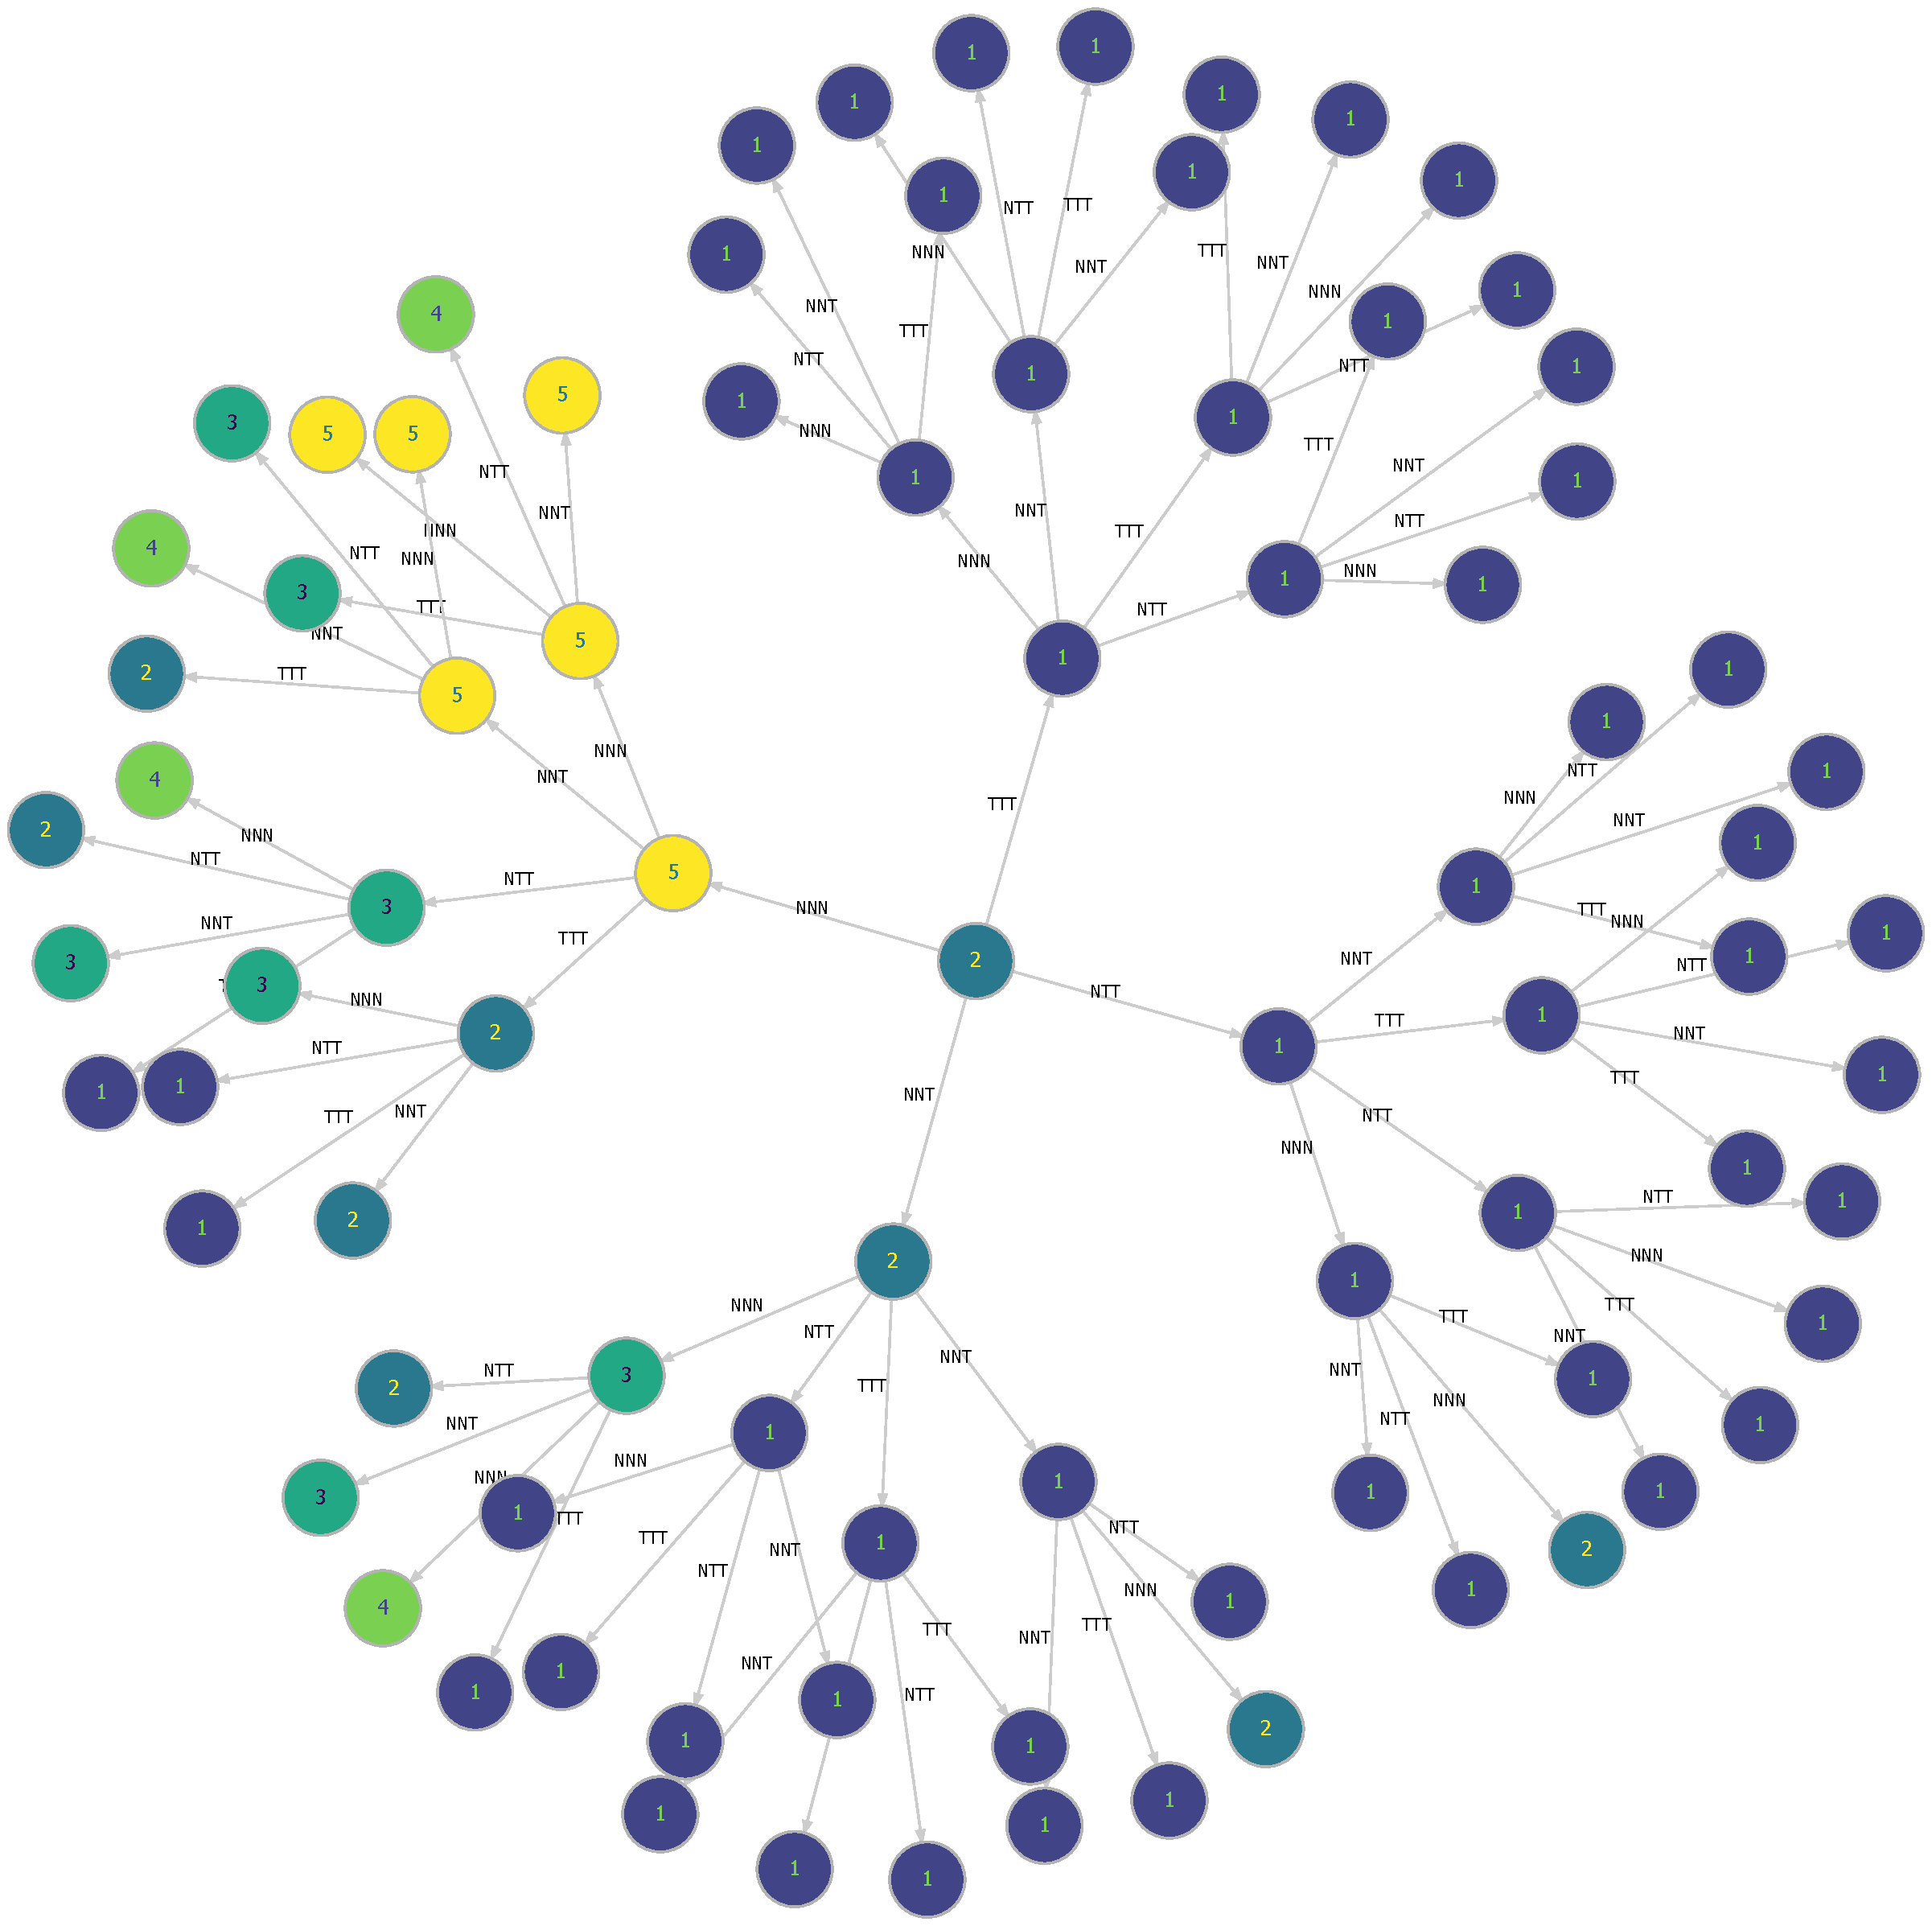
\includegraphics[width=\textwidth]{TITE-DTP-InitialExampleDTPNode}
\end{figure}

\begin{figure}[h!]
	\centering
	\caption[Initial DTP flow plot.]{Node plot of the initial DTP for the first three cohorts of our example CRM.}
	\label{fig_tite-dtp:InitialDTPExampleFlow}
	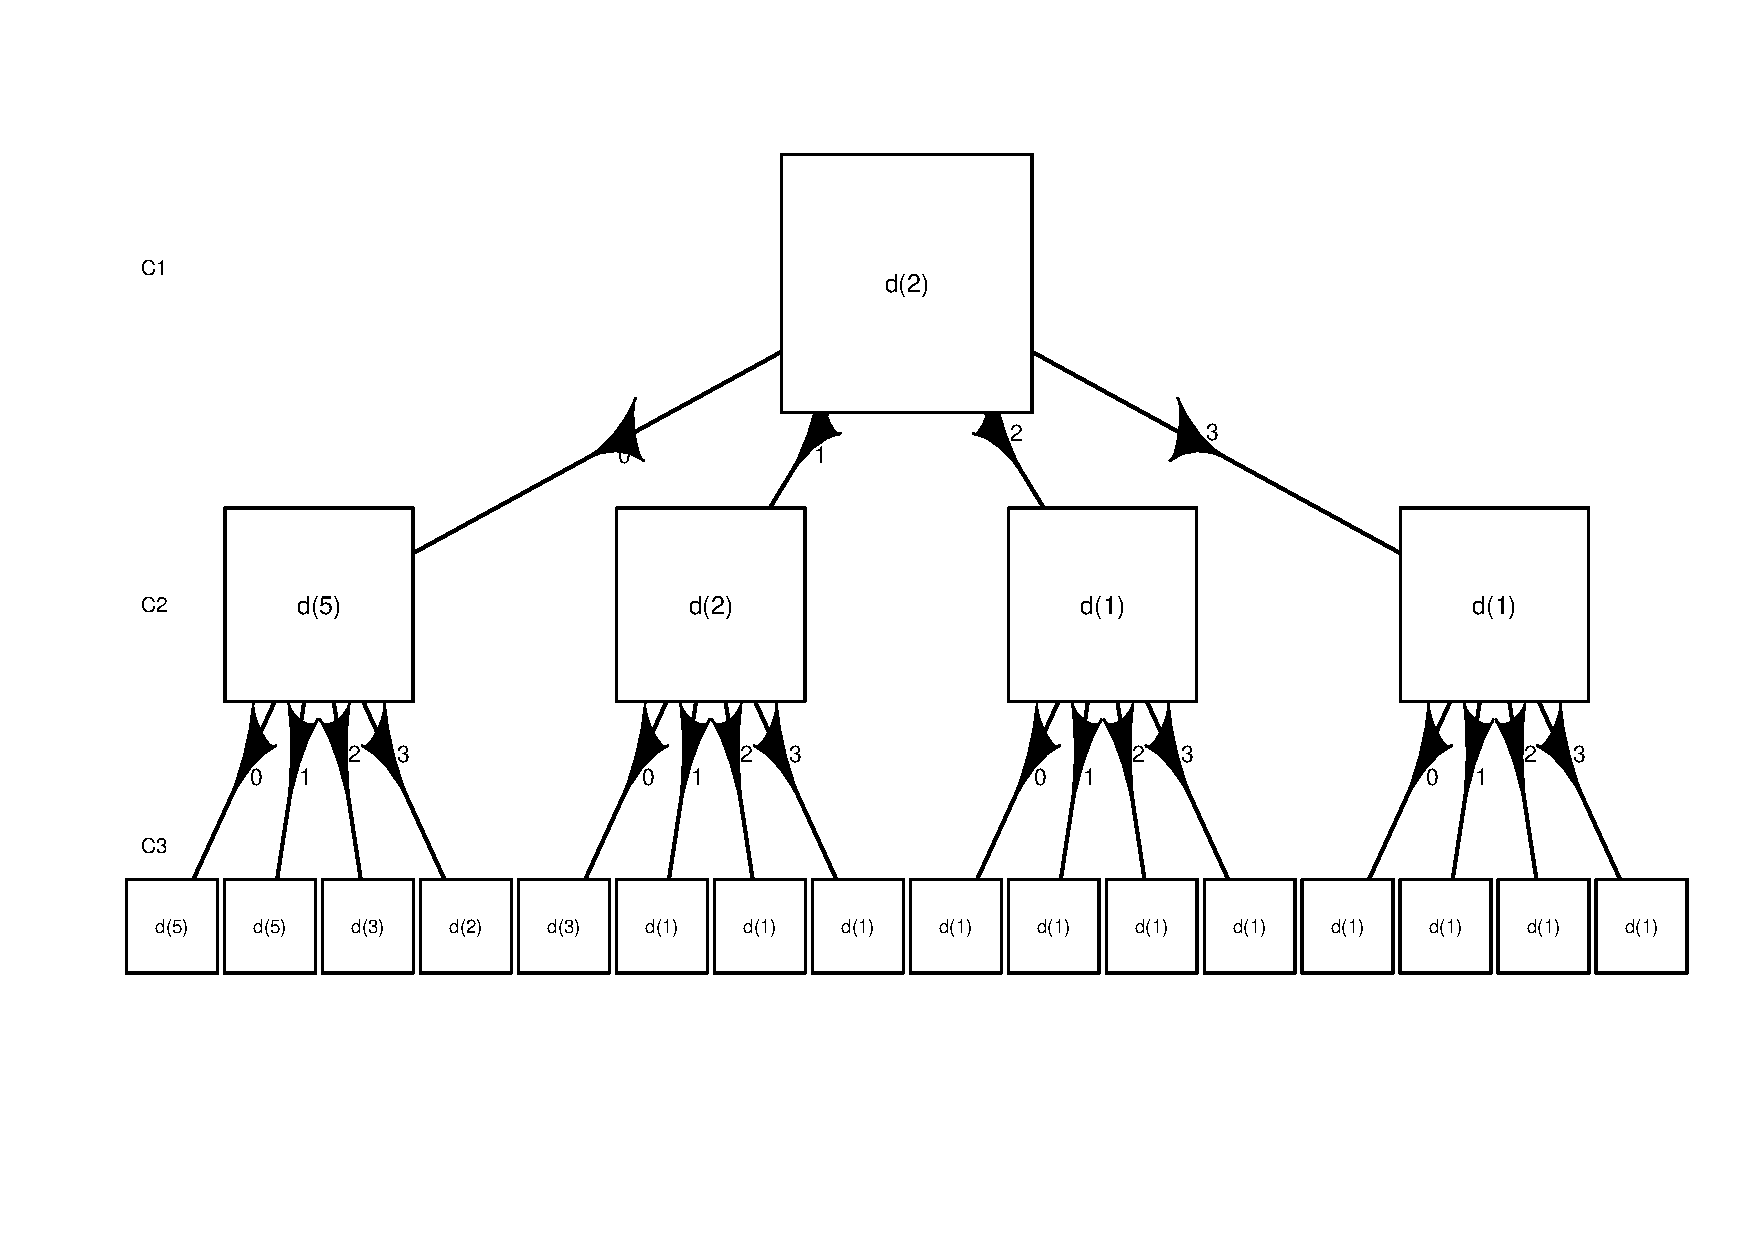
\includegraphics[width=\textwidth]{TITE-DTP-InitialExampleDTPFlow}
\end{figure}

From Table \ref{tab_tite-dtp:InitialDTPExample}, looking at pathways 33-64, we can see that if there are two or more toxicities in the first cohort the CRM will always de-escalate the dose and if there are one or more toxicities in the next two cohorts it will stay at dose-level 1. We can also see from pathways 17-32 if we observe a toxicity in the first cohort we will stay at the same dose-level for the next cohort. If no toxicities occur we escalate straight to the highest dose. 

Figure \ref{fig_tite-dtp:InitialDTPExampleNode} also shows the same information. The central node represents the starting dose and first cohort, from here we have 4 branches showing the various outcomes and which dose-level is allocated to the next cohort. A quick glance at the case where each patient in the first cohort experience a DLT (TTT) we see that subsequent cohorts are all allocated to dose-level 1 regardless of their outcomes. Similarly, for when two patients from the first cohort experience DLTs (NTT) all resulting branches show that dose-level 1 would be selected except in one case where no further DLTs occur and the CRM would escalate back to the starting dose. When one DLT occurs in the first cohort (NNT), we remain at the same dose-level. Looking at these branches if one or more DLTs are experienced in the next cohorts the dose-level is de-escalated, there is only potential for escalation in the scenario where no further DLTs occur. For the case when no DLTs occur (NNN) we see the dose for the second cohort escalated to dose-level 5. At this point if the second cohort experiences 3 DLTs the CRM will de-escalate to dose-level 2, if there are only 2 DLTs the CRM goes to dose-level 3 and one ore less DLTs and the next cohort will remain at dose-level 5. The flow plot, Figure \ref{fig_tite-dtp:InitialDTPExampleFlow}, only shows outcomes up to the third cohort but can be interpreted in a similar manner to the node plot.

In combination with operating characteristics from simulations, DTPs can be used to facilitate discussions to see if the CRM can be better calibrated and is behaving in an optimal manner. In our example here there may be a few obvious things that would concern clinicians, the first being that we skip doses when escalating and secondly that in the cases where lots of toxicity occurs recruitment continues. To remedy this we can include a rule not to skip untried doses and add a safety rule if to stop the trial if too many toxicities occur at the lowest dose. 

In a Bayesian setting an appropriate method to stop early would be to test the posterior distribution for the probability of toxicity. For our example here we will stop if there is at least a 90\% probability that the toxicity rate is 10\% greater than the target level at the lowest dose. This can be expressed as $P($true DLT rate at $d_1 > 0.25 + 0.1$ | observed data and prior information $) > 0.9$. 

With the addition of these two rules the DTPs can be updated, and in parallel further simulations can be produced. Table \ref{tab_tite-dtp:UpdatedDTPExample} shows the pathways for the first three cohorts. The node and flow plots were also updated, Figure \ref{fig_tite-dtp:UpdatedDTPExampleNode} and \ref{fig_tite-dtp:UpdatedDTPExampleFlow} respectively. Since we included a rule to stop in the case of excess toxicity we see a number of pathways terminate early so overall there are less pathways compared to the initial set that were produced. Here we see six different branches where its recommended that the trial stop early (pathways 32, 44, 45, 53, 54, 55 Table \ref{tab_tite-dtp:UpdatedDTPExample}). This can also be seen in Figure \ref{fig_tite-dtp:UpdatedDTPExampleNode}, we can also see three of these nodes recommend stopping before recruiting a third cohort. Using the flow plot, Figure \ref{fig_tite-dtp:UpdatedDTPExampleFlow}, we can clearly see that stopping is suggested when five out of the first six patients experience a DLT. Also, escalation of doses no longer skips dose-levels. With these new rules we observe that if there are no DLTs in the first cohort the dose for the next cohort is dose-level 3 and not 5. We still observe that one toxicity in the first cohort leads to recruiting the next cohort at that same dose-level and with two or more toxicities de-escalation occurs. 

\begin{table}[h!]
	
	\caption{\label{tab_tite-dtp:UpdatedDTPExample}Updated DTPs for the first three cohorts of our example CRM with additional rules.}
	\centering
	\resizebox{\linewidth}{!}{
		\fontsize{4}{3}\selectfont
		\begin{tabular}[t]{cccccccc}
			\toprule
			\multicolumn{1}{c}{} & \multicolumn{2}{c}{Cohort 1} & \multicolumn{2}{c}{Cohort 2} & \multicolumn{2}{c}{Cohort 3} & \multicolumn{1}{c}{Cohort 4} \\
			\cmidrule(l{3pt}r{3pt}){2-3} \cmidrule(l{3pt}r{3pt}){4-5} \cmidrule(l{3pt}r{3pt}){6-7} \cmidrule(l{3pt}r{3pt}){8-8}
			Pathway & Dose & Outcomes & Dose & Outcomes & Dose & Outcomes & Dose\\
			\midrule
			\cellcolor{gray!6}{1} & \cellcolor{gray!6}{2} & \cellcolor{gray!6}{NNN} & \cellcolor{gray!6}{3} & \cellcolor{gray!6}{NNN} & \cellcolor{gray!6}{4} & \cellcolor{gray!6}{NNN} & \cellcolor{gray!6}{5}\\
			2 & 2 & NNN & 3 & NNN & 4 & NNT & 5\\
			\cellcolor{gray!6}{3} & \cellcolor{gray!6}{2} & \cellcolor{gray!6}{NNN} & \cellcolor{gray!6}{3} & \cellcolor{gray!6}{NNN} & \cellcolor{gray!6}{4} & \cellcolor{gray!6}{NTT} & \cellcolor{gray!6}{4}\\
			4 & 2 & NNN & 3 & NNN & 4 & TTT & 3\\
			\cellcolor{gray!6}{5} & \cellcolor{gray!6}{2} & \cellcolor{gray!6}{NNN} & \cellcolor{gray!6}{3} & \cellcolor{gray!6}{NNT} & \cellcolor{gray!6}{3} & \cellcolor{gray!6}{NNN} & \cellcolor{gray!6}{4}\\
			6 & 2 & NNN & 3 & NNT & 3 & NNT & 3\\
			\cellcolor{gray!6}{7} & \cellcolor{gray!6}{2} & \cellcolor{gray!6}{NNN} & \cellcolor{gray!6}{3} & \cellcolor{gray!6}{NNT} & \cellcolor{gray!6}{3} & \cellcolor{gray!6}{NTT} & \cellcolor{gray!6}{2}\\
			8 & 2 & NNN & 3 & NNT & 3 & TTT & 1\\
			\cellcolor{gray!6}{9} & \cellcolor{gray!6}{2} & \cellcolor{gray!6}{NNN} & \cellcolor{gray!6}{3} & \cellcolor{gray!6}{NTT} & \cellcolor{gray!6}{2} & \cellcolor{gray!6}{NNN} & \cellcolor{gray!6}{3}\\
			10 & 2 & NNN & 3 & NTT & 2 & NNT & 2\\
			\cellcolor{gray!6}{11} & \cellcolor{gray!6}{2} & \cellcolor{gray!6}{NNN} & \cellcolor{gray!6}{3} & \cellcolor{gray!6}{NTT} & \cellcolor{gray!6}{2} & \cellcolor{gray!6}{NTT} & \cellcolor{gray!6}{1}\\
			12 & 2 & NNN & 3 & NTT & 2 & TTT & 1\\
			\cellcolor{gray!6}{13} & \cellcolor{gray!6}{2} & \cellcolor{gray!6}{NNN} & \cellcolor{gray!6}{3} & \cellcolor{gray!6}{TTT} & \cellcolor{gray!6}{1} & \cellcolor{gray!6}{NNN} & \cellcolor{gray!6}{2}\\
			14 & 2 & NNN & 3 & TTT & 1 & NNT & 1\\
			\cellcolor{gray!6}{15} & \cellcolor{gray!6}{2} & \cellcolor{gray!6}{NNN} & \cellcolor{gray!6}{3} & \cellcolor{gray!6}{TTT} & \cellcolor{gray!6}{1} & \cellcolor{gray!6}{NTT} & \cellcolor{gray!6}{1}\\
			16 & 2 & NNN & 3 & TTT & 1 & TTT & 1\\
			\cellcolor{gray!6}{17} & \cellcolor{gray!6}{2} & \cellcolor{gray!6}{NNT} & \cellcolor{gray!6}{2} & \cellcolor{gray!6}{NNN} & \cellcolor{gray!6}{3} & \cellcolor{gray!6}{NNN} & \cellcolor{gray!6}{4}\\
			18 & 2 & NNT & 2 & NNN & 3 & NNT & 3\\
			\cellcolor{gray!6}{19} & \cellcolor{gray!6}{2} & \cellcolor{gray!6}{NNT} & \cellcolor{gray!6}{2} & \cellcolor{gray!6}{NNN} & \cellcolor{gray!6}{3} & \cellcolor{gray!6}{NTT} & \cellcolor{gray!6}{2}\\
			20 & 2 & NNT & 2 & NNN & 3 & TTT & 1\\
			\cellcolor{gray!6}{21} & \cellcolor{gray!6}{2} & \cellcolor{gray!6}{NNT} & \cellcolor{gray!6}{2} & \cellcolor{gray!6}{NNT} & \cellcolor{gray!6}{1} & \cellcolor{gray!6}{NNN} & \cellcolor{gray!6}{2}\\
			22 & 2 & NNT & 2 & NNT & 1 & NNT & 1\\
			\cellcolor{gray!6}{23} & \cellcolor{gray!6}{2} & \cellcolor{gray!6}{NNT} & \cellcolor{gray!6}{2} & \cellcolor{gray!6}{NNT} & \cellcolor{gray!6}{1} & \cellcolor{gray!6}{NTT} & \cellcolor{gray!6}{1}\\
			24 & 2 & NNT & 2 & NNT & 1 & TTT & 1\\
			\cellcolor{gray!6}{25} & \cellcolor{gray!6}{2} & \cellcolor{gray!6}{NNT} & \cellcolor{gray!6}{2} & \cellcolor{gray!6}{NTT} & \cellcolor{gray!6}{1} & \cellcolor{gray!6}{NNN} & \cellcolor{gray!6}{1}\\
			26 & 2 & NNT & 2 & NTT & 1 & NNT & 1\\
			\cellcolor{gray!6}{27} & \cellcolor{gray!6}{2} & \cellcolor{gray!6}{NNT} & \cellcolor{gray!6}{2} & \cellcolor{gray!6}{NTT} & \cellcolor{gray!6}{1} & \cellcolor{gray!6}{NTT} & \cellcolor{gray!6}{1}\\
			28 & 2 & NNT & 2 & NTT & 1 & TTT & 1\\
			\cellcolor{gray!6}{29} & \cellcolor{gray!6}{2} & \cellcolor{gray!6}{NNT} & \cellcolor{gray!6}{2} & \cellcolor{gray!6}{TTT} & \cellcolor{gray!6}{1} & \cellcolor{gray!6}{NNN} & \cellcolor{gray!6}{1}\\
			30 & 2 & NNT & 2 & TTT & 1 & NNT & 1\\
			\cellcolor{gray!6}{31} & \cellcolor{gray!6}{2} & \cellcolor{gray!6}{NNT} & \cellcolor{gray!6}{2} & \cellcolor{gray!6}{TTT} & \cellcolor{gray!6}{1} & \cellcolor{gray!6}{NTT} & \cellcolor{gray!6}{1}\\
			32 & 2 & NNT & 2 & TTT & 1 & TTT & STOP\\
			\cellcolor{gray!6}{33} & \cellcolor{gray!6}{2} & \cellcolor{gray!6}{NTT} & \cellcolor{gray!6}{1} & \cellcolor{gray!6}{NNN} & \cellcolor{gray!6}{1} & \cellcolor{gray!6}{NNN} & \cellcolor{gray!6}{2}\\
			34 & 2 & NTT & 1 & NNN & 1 & NNT & 1\\
			\cellcolor{gray!6}{35} & \cellcolor{gray!6}{2} & \cellcolor{gray!6}{NTT} & \cellcolor{gray!6}{1} & \cellcolor{gray!6}{NNN} & \cellcolor{gray!6}{1} & \cellcolor{gray!6}{NTT} & \cellcolor{gray!6}{1}\\
			36 & 2 & NTT & 1 & NNN & 1 & TTT & 1\\
			\cellcolor{gray!6}{37} & \cellcolor{gray!6}{2} & \cellcolor{gray!6}{NTT} & \cellcolor{gray!6}{1} & \cellcolor{gray!6}{NNT} & \cellcolor{gray!6}{1} & \cellcolor{gray!6}{NNN} & \cellcolor{gray!6}{1}\\
			38 & 2 & NTT & 1 & NNT & 1 & NNT & 1\\
			\cellcolor{gray!6}{39} & \cellcolor{gray!6}{2} & \cellcolor{gray!6}{NTT} & \cellcolor{gray!6}{1} & \cellcolor{gray!6}{NNT} & \cellcolor{gray!6}{1} & \cellcolor{gray!6}{NTT} & \cellcolor{gray!6}{1}\\
			40 & 2 & NTT & 1 & NNT & 1 & TTT & 1\\
			\cellcolor{gray!6}{41} & \cellcolor{gray!6}{2} & \cellcolor{gray!6}{NTT} & \cellcolor{gray!6}{1} & \cellcolor{gray!6}{NTT} & \cellcolor{gray!6}{1} & \cellcolor{gray!6}{NNN} & \cellcolor{gray!6}{1}\\
			42 & 2 & NTT & 1 & NTT & 1 & NNT & 1\\
			\cellcolor{gray!6}{43} & \cellcolor{gray!6}{2} & \cellcolor{gray!6}{NTT} & \cellcolor{gray!6}{1} & \cellcolor{gray!6}{NTT} & \cellcolor{gray!6}{1} & \cellcolor{gray!6}{NTT} & \cellcolor{gray!6}{1}\\
			44 & 2 & NTT & 1 & NTT & 1 & TTT & STOP\\
			\cellcolor{gray!6}{45} & \cellcolor{gray!6}{2} & \cellcolor{gray!6}{NTT} & \cellcolor{gray!6}{1} & \cellcolor{gray!6}{TTT} & \cellcolor{gray!6}{STOP} & \cellcolor{gray!6}{NA} & \cellcolor{gray!6}{STOP}\\
			46 & 2 & TTT & 1 & NNN & 1 & NNN & 1\\
			\cellcolor{gray!6}{47} & \cellcolor{gray!6}{2} & \cellcolor{gray!6}{TTT} & \cellcolor{gray!6}{1} & \cellcolor{gray!6}{NNN} & \cellcolor{gray!6}{1} & \cellcolor{gray!6}{NNT} & \cellcolor{gray!6}{1}\\
			48 & 2 & TTT & 1 & NNN & 1 & NTT & 1\\
			\cellcolor{gray!6}{49} & \cellcolor{gray!6}{2} & \cellcolor{gray!6}{TTT} & \cellcolor{gray!6}{1} & \cellcolor{gray!6}{NNN} & \cellcolor{gray!6}{1} & \cellcolor{gray!6}{TTT} & \cellcolor{gray!6}{1}\\
			50 & 2 & TTT & 1 & NNT & 1 & NNN & 1\\
			\cellcolor{gray!6}{51} & \cellcolor{gray!6}{2} & \cellcolor{gray!6}{TTT} & \cellcolor{gray!6}{1} & \cellcolor{gray!6}{NNT} & \cellcolor{gray!6}{1} & \cellcolor{gray!6}{NNT} & \cellcolor{gray!6}{1}\\
			52 & 2 & TTT & 1 & NNT & 1 & NTT & 1\\
			\cellcolor{gray!6}{53} & \cellcolor{gray!6}{2} & \cellcolor{gray!6}{TTT} & \cellcolor{gray!6}{1} & \cellcolor{gray!6}{NNT} & \cellcolor{gray!6}{1} & \cellcolor{gray!6}{TTT} & \cellcolor{gray!6}{STOP}\\
			54 & 2 & TTT & 1 & NTT & STOP & NA & STOP\\
			\cellcolor{gray!6}{55} & \cellcolor{gray!6}{2} & \cellcolor{gray!6}{TTT} & \cellcolor{gray!6}{1} & \cellcolor{gray!6}{TTT} & \cellcolor{gray!6}{STOP} & \cellcolor{gray!6}{NA} & \cellcolor{gray!6}{STOP}\\
			\bottomrule
	\end{tabular}}
\end{table}

\begin{figure}[h!]
	\centering
	\caption[Updated DTP node plot.]{Updated DTP node plot for the first three cohorts of our example CRM with additional rules.}
	\label{fig_tite-dtp:UpdatedDTPExampleNode}
	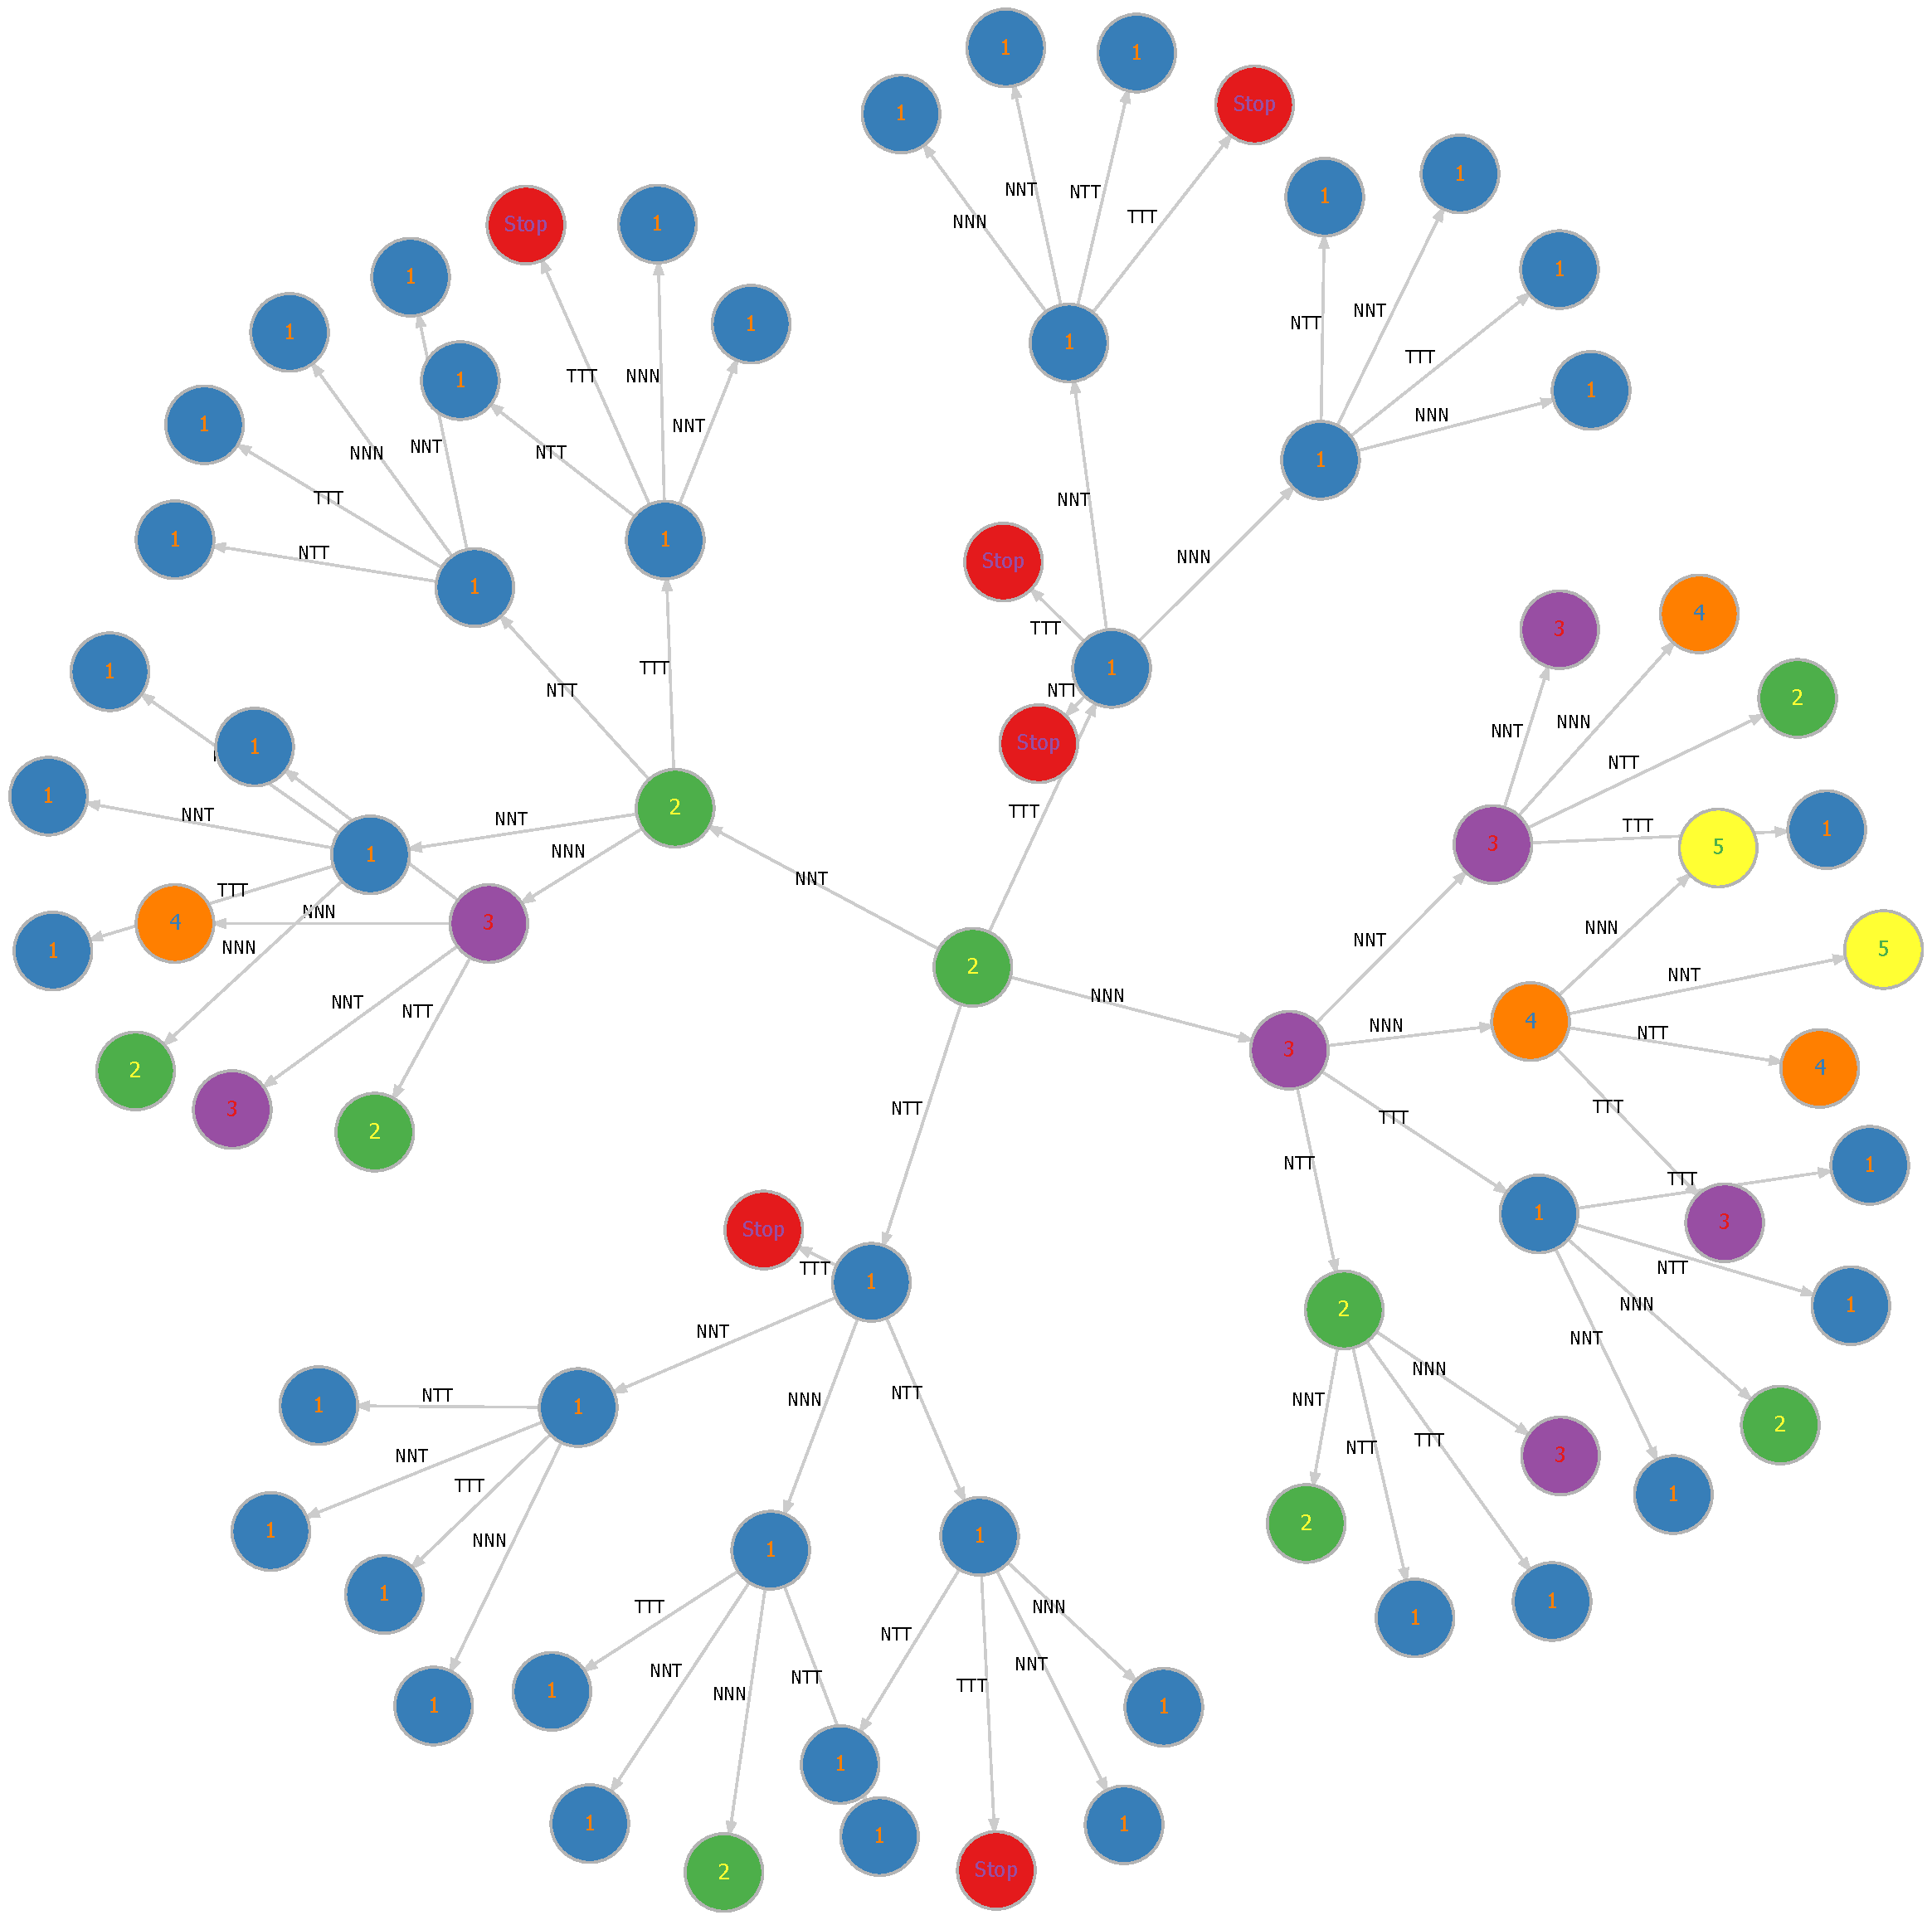
\includegraphics[width=\textwidth]{TITE-DTP-UpdatedExampleDTPNode}
\end{figure}

\begin{figure}[h!]
	\centering
	\caption[Updated DTP flow plot.]{Node plot of the updated DTP for the first three cohorts of our example CRM with additional rules.}
	\label{fig_tite-dtp:UpdatedDTPExampleFlow}
	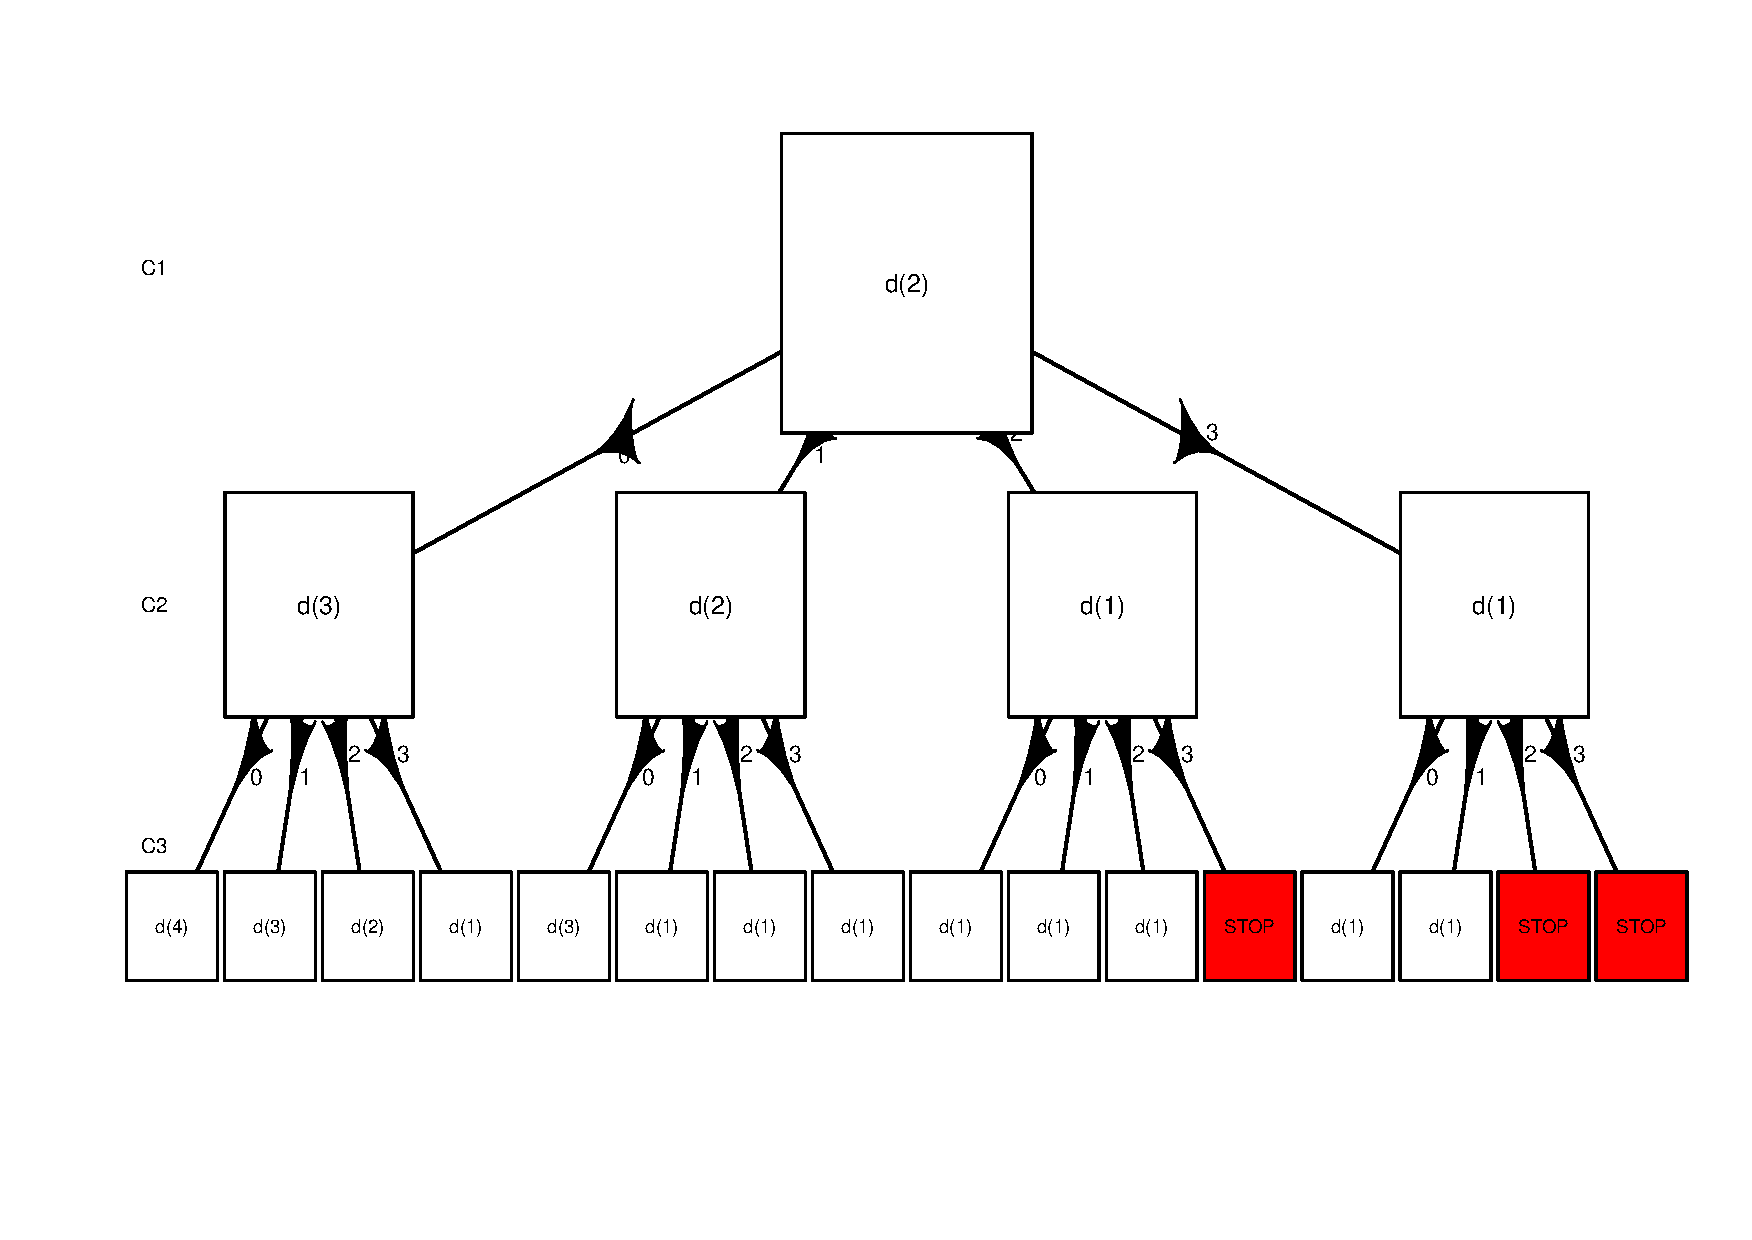
\includegraphics[width=\textwidth]{TITE-DTP-UpdatedExampleDTPFlow}
\end{figure}

At this stage, further discussions could be held about the updated DTPs and simulations. Here there, may be more subtle points to discuss such as the parameters of the stopping rule. Dependent on the clinical rational investigators may be inclined to impose either looser or stricter stopping rules. In our example here this can be done by altering the threshold values in our test of the posterior distribution of the probability of toxicity. 

We also see in pathway 2 that an escalation occurs after observing a toxicity in the previous cohort. This shows our design to be incoherent. A CRM design is considered coherent if escalation only occurs when the previous cohort experiences no DLTs and de-escalation only occurs when a DLT has been observed in the previous cohort. This property limits the risk of unnecessarily exposing patients to toxic doses whilst also ensuring patients get treated at a reasonable dose within the safety limit \cite{cheungDoseFindingContinual2011}. This became an issue due to the rule we enforced not to skip doses in escalation, the previous design without this rule was in fact coherent. Further rules could be added to ensure the design remains coherent such that escalation will only take place if the previous cohort experience no DLTs likewise, de-escalation will only occur if the previous cohort did experience DLTs. 

Here we have highlighted the ways in which DTPs can be utilised during the initial stages of setting up a trial. Due to our example there we some obvious changes that could be implemented into our suggested design. However, this was just to illustrate what the pathways look like and how they can be used to facilitate discussions with the relevant clinicians and the trials team. Although we just looked at DTPs any changes being made to the design should also take into account results from the simulations. CRM designs may not be intuitively understood by clinicians but DTPs should help make them more accessible. Next we will look at how DTPs can be used during a trial.  
%-----------------------------------
%	SUBSECTION 2
%-----------------------------------

\subsection{DTPs as an analysis tool}